\documentclass[12pt,a4paper]{book}
\usepackage[minitoc]{teach}
\usepackage[utf8]{inputenc}
\usepackage[french]{babel}
\usepackage[T1]{fontenc}
\usepackage{amsmath}
\usepackage{amsfonts}
\usepackage{amssymb}
\usepackage{graphicx}
\renewcommand{\headrulewidth}{0pt}
\renewcommand{\footrulewidth}{0pt}
\fancyfoot[C]{\thepage}


\author{YAWO Kossi Atsu}
\newcommand{\prof}{YAWO Kossi Atsu}
\newcommand{\matiere}{MATHEMATIQUES}
\newcommand{\classe}{4$^{ème}$}
\title{Mes devoirs de Mathématiques}
\begin{document}
\begin{devoir}{DEVOIR SURVEILLE DU PREMIER TRIMESTRE}{\matiere}{\classe}{2}{2H}{13 novembre 2019}{\prof}
\begin{exo}[4]
Une salle de concert peut contenir $600$ personnes. Il y a $x$ places assises et les
autres sont debout. Les places debout coûtent $5000 F CFA$ et les places assises $10000 F CFA$.
\begin{enumerate}
\item Que représentent les expressions
suivantes : 
\begin{enumerate}
\item $600-x$ ?
\item $10000x$ ?
\item $5000\times(600-x)$ ?
\end{enumerate}
\item Exprime, en fonction de $x$, la recette totale en francs CFA si toutes les places sont prises.
\item Calcule cette recette si $x = 200$.
\end{enumerate}
\competence{•}{4}
\end{exo}

\vspace{1cm}

\begin{exo}[6]
\begin{enumerate}
\item Calcule la somme algébrique suivante:
$A=(-4,2)-(-11,8)+(-9,4)+(+13,6)-(-5,6)$
\competence{•}{1}
\item Reproduis puis complète le tableau suivant:\\
\begin{tabular}{|c|c|c|c|}
\hline 
a & b & c & $a \times b \times c$ \\ 
\hline 
-2 & +3 & -5 & • \\ 
\hline 
-1 & -6 & -2 & • \\ 
\hline 
3 & • & -4 & 24 \\ 
\hline 
\end{tabular} 
\competence{•}{1.5}
\item Développe les produits suivants:
$B=(x-2)^2$  \qquad ; \qquad $C=(x-2)(3x+5)-2x(5x+7)$
\item Écris les sommes suivantes sous la forme de produit:
$D=x^2-49$  \qquad ; \qquad $E=(x-2)(3x+5)-(3x+5)(5x+7)$
\competence{Développer}{1}
\item Calcule de manière performante:
$19^2$ \qquad ; \qquad $29^2$ \qquad ; \qquad $29 \times 31$ 
\competence{factoriser}{1}
\competence{•}{1.5}
\end{enumerate}

\end{exo}

\vspace{1cm}

\begin{exo}[5]
On donne un segment $[AB]$ de longueur 5cm et désire construire à la règle et au compas uniquement, un triangle ABC rectangle en A et dont la hauteur $[AH]$ mesure 4cm.
\begin{enumerate}
\item Donne un programme de construction de cette figure.
\item Réalise la construction en respectant le programme que tu as établi.
\end{enumerate} 
\competence{•}{5}
\end{exo}

\vspace{1cm}

\begin{exo}[5]
$TSU$ est un triangle en $S$. La médiatrice de $[SU]$ coupe $(SU)$ en V et $(TU)$ en $W$. 
\begin{enumerate}
\item Fais une figure.
\item Démontre que les droites $(VW)$ et $(TS)$ sont parallèles.
\item Démontre que $SUW$ est un triangle isocèle.
\end{enumerate}
\end{exo}
\competence{•}{5}

\tableofcompetences
\end{devoir}


\newpage
\begin{td}{\matiere}{\classe}{23 novembre 2019}{\prof}
\begin{exo}
$\mathcal{(C)}$ est un cercle de centre $O$ et $\mathcal{(C')}$ est un cercle de centre $O'$ tels que $\mathcal{(C)}$ et $\mathcal{(C')}$ n'ont pas le même rayon et se coupent en $A$ et $B$. Le point $D$ est le symétrique du point $A$ par rapport à O et le point E, le symétrique de $A$ par rapport à $O'$.
\begin{enumerate}
\item Fais une figure.
\item Démontre que les points $A$, $B$ et $C$ sont alignés.
\item Démontre que les droites $(OO')$ et $(DE)$ sont parallèles.
\end{enumerate}
\end{exo}

\vspace{1cm}
\begin{exo}
On donne la droite $(D)$, un point $H$ appartenant à $(D)$ et un point $A$
n'appartenant pas à $(D)$.\\
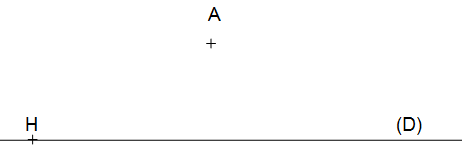
\includegraphics[scale=0.9]{images/td1img1.png}
\par
On désire placer le point M appartenant à $(D)$ tel que $MH=MA$ en utilisant uniquement le compas et la règle non graduée.
\begin{enumerate}
\item Explique comment tu pourras procéder.
\item Écris ensuite un programme de construction.
\item Réalise la construction.
\end{enumerate}
\end{exo}

\vspace{1cm}

\begin{exo}

\end{exo}

\vspace{1cm}

\begin{exo}
\begin{enumerate}
\item Développe les produits suivants:
$B=(3x-2)(3x+2)$  \qquad ; \qquad $C=(x-72)(x+5)-4x(5x+7)$
\item Écris les sommes suivantes sous la forme de produit:
$D=9x^2-16$  \qquad ; \qquad $E=(x-2)(3x+5)-(3x+5)(5x+7)$
\item Calcule de manière performante:
$29^2$ \qquad ; \qquad $31^2$ \qquad ; \qquad $29 \times 31$ 
\end{enumerate}
\end{exo}
\end{td}

\newpage
\begin{devoir}{COMPOSITION DU PREMIER TRIMESTRE}{\matiere}{\classe}{2}{2H}{13 décembre 2019}{\prof}
\begin{exo}[3]
\begin{multicols}{2}
Voici un programme de calcul:
\begin{remslist}
\item Choisir un nombre
\item Tripler ce nombre
\item Ajouter 4 au résultat
\item Doubler le tout
\item Retrancher le produit du nombre de départ par six
\end{remslist}
\begin{enumerate}
\item Qu'obtient-on en choisissant 7 comme nombre de départ?
\item Qu'obtient-on en choisissant -5 comme nombre de départ?
\item Démontre que l'on obtient toujours le même résultat, que tu préciseras, quel que soit le nombre choisi au départ.
\end{enumerate}
\end{multicols}
\competence{•}{3}
\end{exo}

\totalexo

\begin{exo}[3]
\begin{multicols}{2}
On donne la droite $(D)$, un point $H$ appartenant à $(D)$ et un point $A$
n'appartenant pas à $(D)$ comme l'indique la figure ci-contre.
On désire placer le point M appartenant à $(D)$ tel que $MH=MA$ en utilisant uniquement le compas et la règle non graduée.
\begin{enumerate}
\item Explique comment tu pourras procéder.
\item Écris ensuite un programme de construction.
\item Réalise la construction.
\end{enumerate}
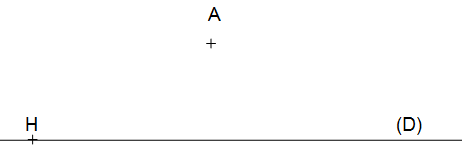
\includegraphics[scale=0.4]{images/td1img1.png}
\end{multicols}
\competence{•}{3}
\end{exo}

\begin{exo}[3]
Komlagan a sept ans de plus que sa petite sœur Adjovi. Dans quatre ans, Komlagan aura le double de l'âge de sa petite sœur.
\begin{enumerate}
\item Quelle équation permet de retrouver l'âge des deux enfants?
\begin{multicols}{4}
\begin{enumerate}
\item $x+11=2(x+4)$
\item $x+7=2x+4$
\item $x-7=2(x+4)$
\item $x+4=2(x-3)$
\end{enumerate}
\end{multicols}
\item Résous cette équation pour déterminer l'âge des deux enfants.
\item Comment peux-tu vérifier les résultats obtenus?
\end{enumerate}

\competence{•}{3}
\end{exo}

\begin{exo}[6]
\begin{multicols}{2}
\begin{enumerate}
\item Développe les produits suivants:\\
$B=(3x-2)(3x+2)$  \qquad ; \qquad $C=(x-72)(x+5)-4x(5x+7)$
\competence{developper}{1}
\item Écris les sommes suivantes sous la forme de produit:
$D=9x^2-16$  \qquad ; \qquad $E=(x-2)(3x+5)-(3x+5)(5x+7)$
\competence{factoriser}{1}
\item Calcule de manière performante:\\
$29^2$ \qquad ; \qquad $31^2$ \qquad ; \qquad $29 \times 31$ \\
\competence{•}{1.5}
\item Compare les fractions suivantes:
\begin{multicols}{2}
\begin{enumerate}
\item $\frac{4}{18}$ et $\frac{2}{9}$
\item $\frac{1}{3}$ et $\frac{1}{5}$
\competence{•}{1}
\end{enumerate}
\end{multicols}
\item Calcule et donne le résultat sous la forme de fraction irréductible:\\
$F=\frac{5}{6}-\frac{1}{3}$ \qquad;\qquad $G=\frac{9}{14}-5$ \qquad;\qquad $H=\frac{1}{6}-\frac{17}{30}+\frac{4}{5}$
\competence{•}{1.5}
\end{enumerate}
\end{multicols}
\end{exo}

\begin{exo}[5]
\begin{multicols}{2}
On considère la figure codée ci-contre.
\begin{enumerate}
\item Recopie puis complète le tableau de correspondance.
\competence{•}{2}
\item Reproduis puis complète la figure en construisant le point F symétrique de T par rapport à H.
\competence{•}{1.5}
\begin{enumerate}
\item Quelle est la nature du quadrilatère ATBF?
\competence{•}{1}
\item Quelle est l'image de F par $S_{(D)}$?\\
\competence{•}{0.5}
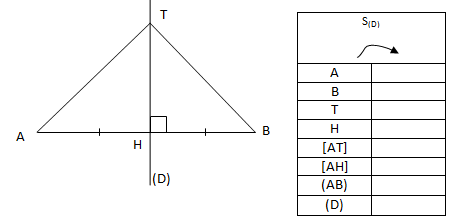
\includegraphics[scale=0.5]{images/compo1img1.png}
\end{enumerate}
\end{enumerate}
\end{multicols}
\end{exo}

\tableofcompetences
\end{devoir}

\newpage
\begin{devoir}{DEVOIR SURVEILLÉ DU DEUXIÈME TRIMESTRE}{\matiere}{\classe}{2}{2H}{12 février 2020}{\prof}
\begin{exo}[7]
\begin{enumerate}
\item Écris sous la forme d'une puissance de 10:\\
100 \qquad ; \qquad 1000 \qquad ; \qquad un milliard \qquad ; \qquad 0,00001.
\item Écris sous la forme de fraction décimale:\\
0,0001 \qquad ; \qquad 0,1.
\item Donne la notation scientifique de chacun des nombres suivants:\\
0,000023 \qquad ; \qquad 45000000 \qquad ; \qquad 12,25 \qquad ; \qquad 175.
\item Écris le résultat sous la forme d'une puissance de 10:\\
$10^4 \times 10^5$ \qquad ; \qquad $1000 \times 10^{-5}$ \qquad ; \qquad $\frac{10^{13}}{10^9}$ \qquad ; \qquad $\frac{(10^{-1})^3}{10^5 \times 10^{-7}}$.
\end{enumerate}
\competence{•}{7}
\end{exo}

\begin{exo}[7]
\begin{enumerate}
\item On donne les expressions littérales suivantes:
$A=2t(t+1)-(3t-2)(t+1)$ \qquad ; \qquad $B=(m+3)^2-16$
\begin{enumerate}
\item Calcule la valeur numérique de B pour $m=-3$
\item Développe et réduis A et B.
\item Factorise A et B.
\end{enumerate}
\item Résoudre les équations ou inéquations suivantes:\\
$(E_1): -3+4x=-5+6x$ \qquad ; \qquad $(E_2): -3+4x=-5+6x$ \qquad ; \qquad $(I_1): -3+4x=-5+6x$ \qquad ; \qquad $(I_2): -3+4x=-5+6x$.
\item \textbf{Problème ouvert}\\
Arthur et Lili choisissent un même nombre. Arthur le multiplie par 10 puis soustrait 3 au résultat obtenu. Lili le multiplie par 7 et ajoute 8 au résultat obtenu. Ils obtiennent tous les deux le même résultat.\\
Quel nombre Arthur et Lili avaient-ils choisi au départ?
\end{enumerate}
\competence{calcul littéral}{7}
\end{exo}

\begin{exo}[4]
ABC est un triangle et M le milieu de $[BC]$. Le point $D$ est le symétrique de $B$ par rapport à $A$ et le point $N$ le symétrique de $M$ par rapport à $A$.
\begin{enumerate}
\item \begin{enumerate}
\item Démontre que le quadrilatère $BMDN$ est un parallélogramme.
\item Déduis-en que: $BM=DN$.
\end{enumerate}
\item \begin{enumerate}
\item Démontre que: $BM=MC$.
\item Déduis-en que: $ND$=$MC$. 
\end{enumerate} 
\item Démontre que les droites $(ND)$ et $(MC)$ sont parallèles puis déduis-en la nature du quadrilatère $MCDN$.
\end{enumerate}
\end{exo}

\begin{exo}[2]
\begin{multicols}{2}
On donne la figure ci-contre. (D) et (L) sont deux droites perpendiculaire en O. A est un point n'appartenant ni à (D), ni à (L).
\begin{enumerate}
\item Construis en utilisant uniquement le compas et la règle non graduée, le point M de (D) et le point N de (L) tels que le point A soit le milieu du segment $[MN]$.
\item Explique ta construction.
\end{enumerate}
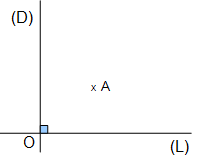
\includegraphics[scale=0.9]{images/dev2_2020_img1.png}
\end{multicols}
\end{exo}

\tableofcompetences
\end{devoir}

\newpage
\begin{td}{\matiere}{\classe}{29 février 2020}{\prof}
\begin{exo}
Écris à l'aide d'une puissance de 10 :
\begin{enumerate}
\item 0,01 \quad ; \quad  0,000 0001 \quad ; \quad  0,001.
\item un dixième \quad ; \quad  un millième \quad ; \quad  un millionième.
\item $\frac{1}{10000}$ \quad ; \quad  $\frac{1}{100000}$ \quad ; \quad  $\frac{1}{10000000}$
\end{enumerate}
\end{exo}

\vspace{0.5cm}

\begin{exo}

Exprime sous la forme d'une puissance de 10 :
\begin{multicols}{4}
$10^5 \times 10^7$\\
$10^4 \times 10^{–12}$\\
$10^{–8} \times 10^9$\\
$10^{–11} \times 10^3 \times 10^2$\\
$10 \times 10^5$\\
$10^{-6} \times 10^6$\\
\end{multicols}
\end{exo}

\vspace{0.5cm}

\begin{exo}
Le cœur humain effectue environ 5 000 battements par heure.
\begin{enumerate}
\item Écrire 5 000 en notation scientifique.
\item Calculer le nombre de battements effectués en un jour, sachant qu'un jour dure 24 heures.
\item Calculer le nombre de battements effectués pendant une vie de 80 ans. On considère qu'une année correspond à 365 jours.
\end{enumerate}
\end{exo}

\vspace{0.5cm}

\begin{exo}
Le cerveau humain est composé de 100 milliards de neurones. À partir de 30 ans, ce nombre de neurones baisse d'environ 100 000 par jour. En considérant qu'une année contient 365 jours, donne l'écriture décimale puis scientifique du nombre de neurones d'un humain de 40 ans.
\end{exo}

\vspace{0.5cm}


\begin{exo}
On donne un rectangle ABCD tel que AB=6cm et BC=4cm.
\begin{enumerate}
\item Quelle est la distance du point A à la droite (CD)?
\item Quelle est la distance du point D à la droite (BC)?
\end{enumerate}
\end{exo}

\vspace{0.5cm}


\begin{exo}
On donne un carré EFGH de côté 5cm de centre O.
\begin{enumerate}
\item Quelle est la distance du point E à la droite (FG)?
\item Mesure la distance du point G à la droite (GF)?
\item Mesure la distance du point O à la droite (HG)?
\end{enumerate}
\end{exo}

\begin{exo}
\begin{multicols}{2}
A et B sont deux points
distincts non diamétralement
opposés d'un cercle $\mathcal{(C)}$ de
centre O. Le point M est le
point d'intersection des
tangentes à $\mathcal{(C)}$ en A et B.
Soit I le milieu du segment
[OM]. Démontre que les
points O, A et B
appartiennent au cercle de
centre I passant par M.\\
\begin{center}
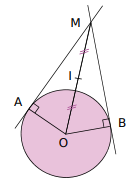
\includegraphics[scale=0.8]{images/td_29_02_2020_img1.png}
\end{center}
\end{multicols}

\end{exo}
\end{td}
\end{document}
